\section{Reconhecimento de padrões}
Para \citeonline{Haykim_ingles}, o reconhecimento de padrões é formalmente definido como o processo que um determinado 
sinal/padrão recebido é classificado para uma das classes predefinidas. A Figura \ref{fig:fluxogramadesign}  exibe um diagrama 
dos componentes de um sistema típico de reconhecimento de padrões. Para entender o problema de projeto de um sistema, é 
necessário o entendimento dos problemas que cada um desses componentes resolve \cite{PatternDuda}.\\

\begin{figure}[H]
  
	\centering
	\caption{Modelo de sistemas de classificações de padrões}
	\label{fig:fluxogramadesign}
	\begin{tikzpicture}[node distance=1cm, >=triangle 60,
	estilo/.style={draw, rectangle, minimum width=5cm, minimum height=1cm, text centered, line width=0.07cm}]
		
		\node[draw=none] 			(A)  {entrada};
		\node[draw, estilo, above=of A] 	(B)  {detecção};
		\node[draw, estilo, above=of B] 	(C)  {segmentação};
		\node[draw, estilo, above=of C] 	(D)  {extração de característica};
		\node[draw=red, estilo, above=of D] 	(E)  {classificação};
		\node[draw, estilo, above=of E] 	(F)  {pós-processamento};
		\node[draw=none, above= of F] 		(G)  {decisão};
		
		\node[draw=none, right=of F, xshift=2cm] 			(H)  {custos};
		\node[draw=none, right=of F, yshift=-1cm,xshift=2cm,align=left] 	(I)  {ajustes para \\ contextos};
		\node[draw=none, right=of E, yshift=-1cm,xshift=2cm,align=left] 	(J)  {ajustes para \\ características 
faltantes};
		
		\draw[->, line width=0.03cm]  (A) -- (B);
		\draw[->, line width=0.03cm]  (B) -- (C);
		\draw[->, line width=0.03cm]  (C) -- (D);
		\draw[->, line width=0.03cm]  (D) -- (E);
		\draw[->, line width=0.03cm]  (E) -- (F);
		\draw[->, line width=0.03cm]  (F) -- (G);
		
		\draw[->, gray, line width=0.03cm]  ($(C.south) + (0.8cm, 0)$) -- ($(B.north) + (0.8cm,0)$);
		\draw[->, gray, line width=0.03cm]  ($(D.south) + (0.8cm, 0)$) -- ($(C.north) + (0.8cm,0)$);
		\draw[->, gray, line width=0.03cm]  ($(E.south) + (0.8cm, 0)$) -- ($(D.north) + (0.8cm,0)$);
		\draw[->, gray, line width=0.03cm]  ($(F.south) + (0.8cm, 0)$) -- ($(E.north) + (0.8cm,0)$);			
		
		\draw[->, red, line width=0.03cm]  (H.west) -- ($(F.east) + (0, 0.2cm)$);
		\draw[->, red, line width=0.03cm]  (I.west) -- ($(F.east) - (0, 0.2cm)$);
		\draw[->, red, line width=0.03cm]  ($(I.west) - (0, 0.2cm)$) -- ($(E.east) + (0, 0.2cm)$);
		\draw[->, red, line width=0.03cm]  (J.west) -- ($(E.east) - (0, 0.2cm)$);
	

	\end{tikzpicture}
	\caption*{Fonte: \citeonline{PatternDuda}.}
\end{figure}


A entrada corresponde a um fenômeno que se deseja avaliar. A detecção converte esse fenômeno em um sinal elétrico, por exemplo, sendo representado por um sensor que no caso do presente trabalho corresponde aos sensores indutivos e acelerômetro. As dificuldades variam de acordo com as limitações sensor, tais como resolução, sensividade, ruído, latência
\cite{PatternDuda}.
  A segmentação separa os objetos detectados pelo sensor de outros objetos ou do cenário. Tomando como base o sinal do acelerômetro, a segmentação é utilizada para separar onde começa o sinal de uma letra e onde termina \cite{PatternDuda}.

  O objetivo tradicional da extração de característica é caracterizar um objeto para ser identificado por valores que podem ser 
  mensurados, em que, esses valores são muito similares para objetos de mesma categoria e muito distantes para objetos de 
  categorias diferentes. Isso leva a ideia de procurar características marcantes que são invariantes para transformações de 
entrada \cite{PatternDuda}.

  O papel do componente classificador em um sistema completo é usar as características escolhidas pela extração e atribuir este 
  objeto a uma classe. Como a classificação perfeita é muitas vezes impossível, uma tarefa mais geral do classificador é definir 
  a porcentagem que um objeto pertença a uma classe \cite{PatternDuda}.

  No pós-processamento são levados em conta as considerações, como os efeitos do contexto e o custo dos erros para determinar a 
ação apropriada. Uma simples medida de desempenho é a porcentagem de erros, a qual se refere a quantidade de classificações para 
uma classificação incorreta. Nesta etapa também pode ser analisada a eficiência de se utilizar múltiplos classificadores, 
adicionando um para a detecção dos gestos por uma câmera, por exemplo \cite{PatternDuda}.
  
  
\section{Redes Neurais}
	Conforme \citeonline{Redes_cursopratico}, redes neurais são estruturas baseadas no sistema nervoso dos seres vivos que possuem a capacidade de armazenar e manter conhecimento.

\subsection{Arquitetura de um neurônio}
O neurônio é uma unidade de processamento de informação fundamental para a operação de uma rede neural, sendo a base para redes neurais artificiais \cite{haykin}. Na Figura \ref{fig:neuronio}, pode-se notar a presença de três elementos: o conjunto de pesos sinápticos; função de ativação; e a junção aditiva.
\begin{figure}[H]
	\vspace{4mm}
	\centering
	\caption{Modelo não linear de um neurônio}
	\label{fig:neuronio}
	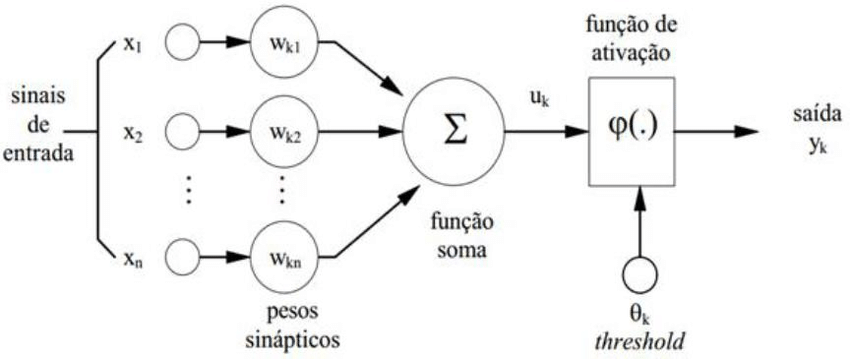
\includegraphics[scale=0.35]{imagens/neuronio}
	\caption*{Fonte: \citeonline[p. 38]{haykin}.}
\end{figure}

De acordo com \citeonline{Redes_cursopratico}, os pesos sinápticos são os valores que servirão para ponderar cada uma das variáveis de entrada da rede, permitindo quantificar as suas relevâncias em relação a funcionalidade do respectivo neurônio. As entradas, após serem ponderadas, são somadas pela junção aditiva ou combinador linear, que é um somador dos valores de entrada ponderados pelos respectivos pesos sinápticos. Esse processo é representado por \cite{haykin}:

\begin{equation}
	u_k = 	\sum_{j=1}^{n}.w_{kj}x_j,
\end{equation}
onde $x_j$ são os sinais de entrada, $w_{kj}$ são os pesos sinápticos, $u_k$ é a saída do combinador linear.

A função de ativação ou função restritiva é aplicada para restringir a amplitude de saída de um neurônio. Tipicamente, a amplitude de saída de um neurônio é escrita como o intervalo unitário fechado $[0, 1]$ ou alternativamente $[-1, 1]$. A função de ativação recebe a saída do combinador linear, conforme \cite{haykin}:

\begin{equation}
	y_l = \varphi(u_k + b_k),
\end{equation}
onde $y_k$ é o sinal de saída do neurônio e $b_k$ é o \textit{bias}. O \textit{bias} tem o efeito de aumentar ou diminuir a entrada líquida da função de ativação \cite{haykin}. O valor do bias é ajustado da mesma forma que os pesos sinápticos. O bias possibilita que um neurônio apresente uma saída não nula mesmo que todas as suas entradas sejam nulas \cite{redesemc}.

\subsection{Funções de ativação}
\label{sec:funcao}
A função de ativação, representada por $\varphi(v)$, define a saída em termos do potencial de ativação $v$. Os principais tipos de funções de ativação consistem da função limiar, representada na Figura \ref{fig:limiar}, e da função sigmoide, mostrada na Figura \ref{fig:sigmoide} \cite{haykin}.

\begin{figure}[H]
	\vspace{4mm}
	\centering
	\caption{Função de ativação limiar}
	\label{fig:limiar}
	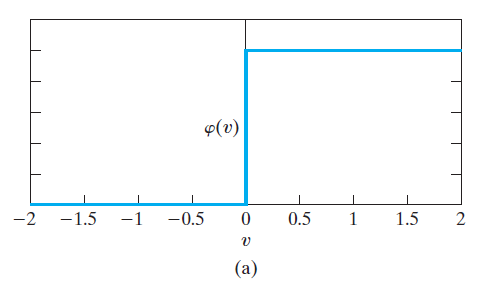
\includegraphics[scale=0.5]{imagens/limiar}
	\caption*{Fonte: \citeonline[p. 39]{haykin}.}
\end{figure}

\begin{figure}[H]
	\vspace{4mm}
	\centering
	\caption{Função de ativação sigmoide}
	\label{fig:sigmoide}
	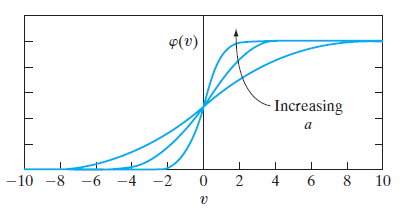
\includegraphics[scale=0.7]{imagens/sigmoide}	
	\caption*{Fonte: \citeonline[p. 39]{haykin}.}
\end{figure}

A função sigmoide é a forma mais comum de função de ativação para a construção de redes neurais artificiais, sendo definida como uma função estritamente crescente que exibe um balanceamento adequado entre comportamento linear e não linear. Dois exemplos de funções de ativação sigmoides são a função logística \cite{haykin}:

\begin{equation}
	\varphi(v) = \frac{1}{1 + exp(-av)},
\end{equation}
e a função tangente hiperbólica:

\begin{equation}
	\varphi(v) = tanh(v).
\end{equation}

\subsection{Arquitetura de uma rede neural}

A arquitetura de uma rede neural artificial define  a forma como seus diversos neurônios estão arranjados, uns em relação aos outros \cite{Redes_cursopratico}.

Nas redes \textit{feedfoward} camada única possuí uma camada de entrada e que se projeta sobre a camada de saída dos neurônios, mas não vice-versa \cite{haykin}. Essa rede é ilustrada na Figura \ref{fig:camadaUnica}.

\begin{figure}[H]
	\vspace{4mm}
	\centering
	\caption{Arquitetura de camada única}
	\label{fig:camadaUnica}
	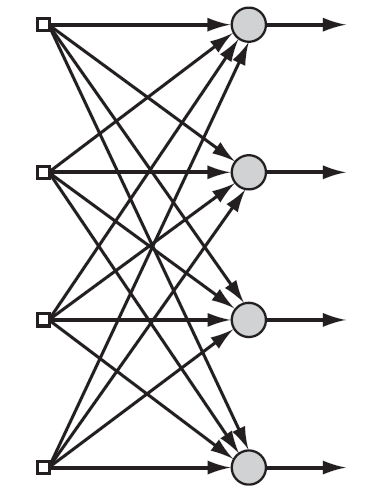
\includegraphics[scale=0.5]{imagens/rede_single}
	\caption*{Fonte: \citeonline[p. 47]{haykin}.}
\end{figure}


De acordo com \citeonline{Redes_cursopratico}, as redes \textit{feedfoward} multicamadas são constituídas de uma ou mais camadas escondidas de neurônios, conforme ilustrado na Figura \ref{fig:camadamultipla}. A função dos neurônios ocultos é intervir entre a entrada externa e a saída da rede de maneira útil. Adicionando-se uma ou mais camadas ocultas, a rede torna-se capaz de extrair características de ordem elevada \cite{haykin}.
\begin{figure}[H]
	\vspace{4mm}
	\centering
	\caption{Arquitetura de múltiplas camadas totalmente conectada}
	\label{fig:camadamultipla}
	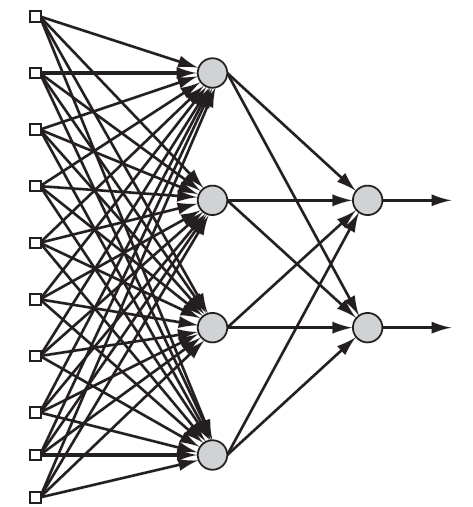
\includegraphics[scale=0.5]{imagens/rede_fully}
	\caption*{Fonte: \citeonline[p. 48]{haykin}.}
\end{figure}

\subsection{Aprendizagem supervisionada}
Conforme \citeonline{Redes_cursopratico}, a estratégia de treinamento supervisionado ou aprendizagem supervisionada consiste em se ter disponível, considerando cada amostra dos sinais de entrada, as respectivas saídas desejadas. Suponha um professor que conhece o ambiente no qual a rede será exposta. Retirando ambos do ambiente e expondo-os ao um vetor de treinamento, o professor é capaz de fornecer a saída correta para a rede neural. Então os parâmetros da rede são ajustados sob a influência combinada do vetor de treinamento e do sinal de erro. O sinal de erro é a diferença entre a resposta desejada e a resposta da rede \cite{haykin}.

Esse ajuste é feito passo a passo, transferindo o conhecimento do professor para a rede, da forma mais completa possível, e quando essa condição é alcançada, pode-se dispensar o professor e deixar a rede neural atuar sozinha \cite{haykin}.

\begin{figure}[H]
	\vspace{4mm}
	\centering
	\caption{Diagrama de aprendizado supervisionado}
	\label{fig:aprendizado}
	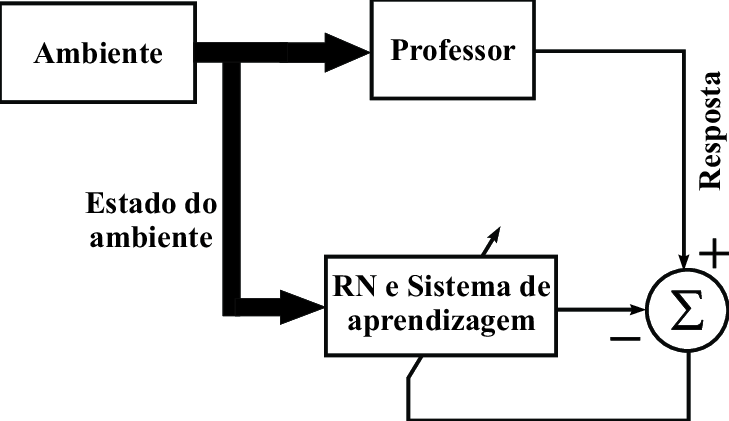
\includegraphics[scale=0.3]{imagens/aprendizado}
	\caption*{Fonte: \citeonline[p. 88]{haykin}.}
\end{figure}

\subsection{O algoritmo \textit{backpropagation}}
Em resumo, o algoritmo de retropropagação pode ser descrito em cinco etapas:

\begin{enumerate}
	\item Inicialização: arbitram-se valores aleatórios aos pesos sinápticos e níveis de \textit{bias}, em uma distribuição uniforme, cuja média deve ser zero \cite{redesemc}.

\item Apresentação dos exemplos: apresenta-se uma época de exemplos a rede. Para cada exemplo, realiza-se uma propagação dos sinais e a retropropagação dos erros com a correção dos pesos e níveis de \textit{bias} \cite{redesemc}.

\item Propagação: aplica-se à camada de entrada da rede o vetor de sinais de entrada e calcula-se a saída para todos os neurônios até a camada de saída, em seguida se calcula o erro para cada neurônio de saída \cite{redesemc}.

\item Retropropagação: calcula-se os ajustes dos pesos daquela camada bem como o \textit{bias}, os quais devem ser somados com os valores atuais. O processo segue até se ajustar os valores de pesos e \textit{bias} da camada de entrada \cite{redesemc}.

\item Iteração: apresentam-se novas épocas de exemplos de treinamento para a rede de forma aleatória até que seja satisfeito o critério de parada \cite{redesemc}.

\end{enumerate}
